\documentclass[twoside]{article}

% Packages required by doxygen
\usepackage{fixltx2e}
\usepackage{calc}
\usepackage{doxygen}
\usepackage[export]{adjustbox} % also loads graphicx
\usepackage{graphicx}
\usepackage[utf8]{inputenc}
\usepackage{makeidx}
\usepackage{multicol}
\usepackage{multirow}
\PassOptionsToPackage{warn}{textcomp}
\usepackage{textcomp}
\usepackage[nointegrals]{wasysym}
\usepackage[table]{xcolor}

% Font selection
\usepackage[T1]{fontenc}
\usepackage[scaled=.90]{helvet}
\usepackage{courier}
\usepackage{amssymb}
\usepackage{sectsty}
\renewcommand{\familydefault}{\sfdefault}
\allsectionsfont{%
  \fontseries{bc}\selectfont%
  \color{darkgray}%
}
\renewcommand{\DoxyLabelFont}{%
  \fontseries{bc}\selectfont%
  \color{darkgray}%
}
\newcommand{\+}{\discretionary{\mbox{\scriptsize$\hookleftarrow$}}{}{}}

% Page & text layout
\usepackage{geometry}
\geometry{%
  a4paper,%
  top=2.5cm,%
  bottom=2.5cm,%
  left=2.5cm,%
  right=2.5cm%
}
\tolerance=750
\hfuzz=15pt
\hbadness=750
\setlength{\emergencystretch}{15pt}
\setlength{\parindent}{0cm}
\setlength{\parskip}{3ex plus 2ex minus 2ex}
\makeatletter
\renewcommand{\paragraph}{%
  \@startsection{paragraph}{4}{0ex}{-1.0ex}{1.0ex}{%
    \normalfont\normalsize\bfseries\SS@parafont%
  }%
}
\renewcommand{\subparagraph}{%
  \@startsection{subparagraph}{5}{0ex}{-1.0ex}{1.0ex}{%
    \normalfont\normalsize\bfseries\SS@subparafont%
  }%
}
\makeatother

% Headers & footers
\usepackage{fancyhdr}
\pagestyle{fancyplain}
\fancyhead[LE]{\fancyplain{}{\bfseries\thepage}}
\fancyhead[CE]{\fancyplain{}{}}
\fancyhead[RE]{\fancyplain{}{\bfseries\leftmark}}
\fancyhead[LO]{\fancyplain{}{\bfseries\rightmark}}
\fancyhead[CO]{\fancyplain{}{}}
\fancyhead[RO]{\fancyplain{}{\bfseries\thepage}}
\fancyfoot[LE]{\fancyplain{}{}}
\fancyfoot[CE]{\fancyplain{}{}}
\fancyfoot[RE]{\fancyplain{}{\bfseries\scriptsize C++ Software transactional Memory }}
\fancyfoot[LO]{\fancyplain{}{\bfseries\scriptsize C++ Software transactional Memory }}
\fancyfoot[CO]{\fancyplain{}{}}
\fancyfoot[RO]{\fancyplain{}{}}
\renewcommand{\footrulewidth}{0.4pt}
\renewcommand{\sectionmark}[1]{%
  \markright{\thesection\ #1}%
}

% Indices & bibliography
\usepackage{natbib}
\usepackage[titles]{tocloft}
\setcounter{tocdepth}{3}
\setcounter{secnumdepth}{5}
\makeindex

% Hyperlinks (required, but should be loaded last)
\usepackage{ifpdf}
\ifpdf
  \usepackage[pdftex,pagebackref=true]{hyperref}
\else
  \usepackage[ps2pdf,pagebackref=true]{hyperref}
\fi
\hypersetup{%
  colorlinks=true,%
  linkcolor=blue,%
  citecolor=blue,%
  unicode%
}

% Custom commands
\newcommand{\clearemptydoublepage}{%
  \newpage{\pagestyle{empty}\cleardoublepage}%
}

\usepackage{caption}
\captionsetup{labelsep=space,justification=centering,font={bf},singlelinecheck=off,skip=4pt,position=top}

%===== C O N T E N T S =====

\begin{document}

% Titlepage & ToC
\hypersetup{pageanchor=false,
             bookmarksnumbered=true,
             pdfencoding=unicode
            }
\pagenumbering{roman}
\begin{titlepage}
\vspace*{7cm}
\begin{center}%
{\Large C++ Software transactional Memory }\\
\vspace*{1cm}
{\large Zoltan Fuzesi}\\
\vspace*{1cm}
{\large C00197361 IT Carlow}\\
\vspace*{1cm}
{\large Supervisor : Joe Kehoe}\\
\vspace*{0.5cm}
{\small Wed Mar 7 2018 21:22:57}\\
\end{center}
\end{titlepage}
\tableofcontents
\pagenumbering{arabic}
\hypersetup{pageanchor=true}

%--- Begin generated contents ---
\section{O\+S\+TM C++ Software Transactional Memory}
\label{index}\hypertarget{index}{}\section{Object Based Software Transactional Memory.}\label{index_OSTM}
\doxyref{O\+S\+TM}{p.}{class_o_s_t_m} is a polymorphic solution to store and manage shared memory spaces within c++ programming context.~\newline
 You can store and managed any kind of object in transactional environment as a shared and protected memory space.\subsection{Brief. Download the zip file from the provided link in the web-\/site, that contains the libostm.\+so, T\+M.\+h, T\+X.\+h, O\+S\+T\+M.\+h files.}\label{index_install_sec}
Unzip the archive file to the desired destination possibly where in you program is stored.\subsection{Step 1\+: Download the archive file.}\label{index_step1}
\subsection{Step 2\+: Unzip in the target destination.}\label{index_step2}
\subsection{Step 3\+: Copy the shared library (libostm.\+so) to the operating system folder where the other shared library are stored.}\label{index_step3}
It will be different destination folder on different platforms. (Linux, Windows, Mac OS) {\tt More Information}\subsection{Step 4\+: Achieve the required class hierarchy between the O\+S\+T\+M library and your own class structure.}\label{index_step4}
Details and instruction of class hierarchy requirements can be found on the web-\/site. www.\+serversite.\+info/ostm\subsection{Step 5\+: Create an executable file as you linking together the T\+M.\+h, T\+X.\+h, O\+S\+T\+M.\+h files with your own files.}\label{index_step5}
\subsection{Step 6\+: Now your application use transactional environment, that guarantees the consistency between object transactions.}\label{index_step6}
\subsection{Step 7\+: Run the application.}\label{index_step7}
Abbreviation for bank names used in the test cases\+:~\newline
 \doxyref{B\+OA}{p.}{class_b_o_a} -\/ Bank of America~\newline
 \doxyref{U\+L\+S\+T\+ER}{p.}{class_u_l_s_t_e_r} -\/ Ulster Bank~\newline
 \doxyref{U\+N\+BL}{p.}{class_u_n_b_l} -\/ United National Bank Limited~\newline
 \doxyref{S\+W\+B\+P\+LC}{p.}{class_s_w_b_p_l_c} -\/ Scottish Windows Bank P\+LC~\newline
 \doxyref{A\+IB}{p.}{class_a_i_b} -\/ Allied Irish Bank~\newline
 \doxyref{B\+OI}{p.}{class_b_o_i} -\/ Bank of Ireland~\newline
 
\section{R\+E\+A\+D\+ME}
\label{md__media_zoltan_Data_00_2018_ITCarlow_00_Modules_06_Project_Documents_Git_Sync_Linux_OSTM_README}
\hypertarget{md__media_zoltan_Data_00_2018_ITCarlow_00_Modules_06_Project_Documents_Git_Sync_Linux_OSTM_README}{}
Usage of the S\+TM library on Linux.~\newline
 In order to use the O\+\_\+\+S\+TM library with any C++ application, it need to be placed to the operation system /usr/lib directory.~\newline

\begin{DoxyEnumerate}
\item Copy lib\+\_\+o\+\_\+stm.\+so file to /usr/lib\+: sudo cp lib\+\_\+o\+\_\+stm.\+so /usr/lib
\item Include the \hyperlink{_t_m_8h_source}{T\+M.\+h} \hyperlink{_t_x_8h_source}{T\+X.\+h} and the \hyperlink{_o_s_t_m_8h_source}{O\+S\+T\+M.\+h} files in your application.~\newline

\item Create Makefile \+: ~\newline
~\newline
 \paragraph*{Makefile.\+mk Documentation$<$br$>$~\newline
}
\end{DoxyEnumerate}

E\+XE =Test~\newline
 CC = g++~\newline
 P\+R\+O\+G\+R\+AM = app~\newline
 C\+F\+L\+A\+GS =-\/std=c++14 -\/pthread ~\newline
 C\+F\+I\+L\+ES = main.\+cpp A\+I\+B.\+cpp U\+L\+S\+T\+E\+R.\+cpp B\+O\+A.\+cpp U\+N\+B\+L.\+cpp S\+W\+B\+P\+L\+C.\+cpp~\newline
 H\+F\+I\+L\+ES = \hyperlink{_t_m_8h_source}{T\+M.\+h} \hyperlink{_t_x_8h_source}{T\+X.\+h} \hyperlink{_o_s_t_m_8h_source}{O\+S\+T\+M.\+h} A\+I\+B.\+h U\+L\+S\+T\+E\+R.\+h B\+O\+A.\+h U\+N\+B\+L.\+h S\+W\+B\+P\+L\+C.\+h~\newline
 ~\newline
~\newline
 all\+:~\newline
 ~\newline
~\newline
 \paragraph*{Rule for S\+H\+A\+R\+ED linking~\newline
}

\+: ~\newline
   $\ast$.cpp -\/I -\/L /usr/lib/lib\+\_\+o\+\_\+stm.so -\/o  ~\newline
 clean\+:~\newline
 rm -\/f $\ast$.o~\newline
 ~\newline

\begin{DoxyEnumerate}
\item Run the application/executable file \+: ./\+Test 
\end{DoxyEnumerate}
\section{Class Index}
\subsection{Class List}
Here are the classes, structs, unions and interfaces with brief descriptions\+:\begin{DoxyCompactList}
\item\contentsline{section}{\hyperlink{class_a_i_b}{A\+IB} }{\pageref{class_a_i_b}}{}
\item\contentsline{section}{\hyperlink{class_b_a_n_k}{B\+A\+NK} }{\pageref{class_b_a_n_k}}{}
\item\contentsline{section}{\hyperlink{class_b_o_a}{B\+OA} }{\pageref{class_b_o_a}}{}
\item\contentsline{section}{\hyperlink{class_b_o_i}{B\+OI} }{\pageref{class_b_o_i}}{}
\item\contentsline{section}{\hyperlink{class_c_a_r_l_o_w___w}{C\+A\+R\+L\+O\+W\+\_\+W} }{\pageref{class_c_a_r_l_o_w___w}}{}
\item\contentsline{section}{\hyperlink{class_c_a_r_p_h_o_n_e___w_a_r_e_h_o_u_s_e}{C\+A\+R\+P\+H\+O\+N\+E\+\_\+\+W\+A\+R\+E\+H\+O\+U\+SE} }{\pageref{class_c_a_r_p_h_o_n_e___w_a_r_e_h_o_u_s_e}}{}
\item\contentsline{section}{\hyperlink{class_d_u_n_d_a_l_k___w}{D\+U\+N\+D\+A\+L\+K\+\_\+W} }{\pageref{class_d_u_n_d_a_l_k___w}}{}
\item\contentsline{section}{\hyperlink{class_k_i_l_k_e_n_n_y___w}{K\+I\+L\+K\+E\+N\+N\+Y\+\_\+W} }{\pageref{class_k_i_l_k_e_n_n_y___w}}{}
\item\contentsline{section}{\hyperlink{class_s_l_i_g_o___w}{S\+L\+I\+G\+O\+\_\+W} }{\pageref{class_s_l_i_g_o___w}}{}
\item\contentsline{section}{\hyperlink{class_s_w_b_p_l_c}{S\+W\+B\+P\+LC} }{\pageref{class_s_w_b_p_l_c}}{}
\item\contentsline{section}{\hyperlink{class_t_a_l_l_a_g_h___w}{T\+A\+L\+L\+A\+G\+H\+\_\+W} }{\pageref{class_t_a_l_l_a_g_h___w}}{}
\item\contentsline{section}{\hyperlink{class_u_l_s_t_e_r}{U\+L\+S\+T\+ER} }{\pageref{class_u_l_s_t_e_r}}{}
\item\contentsline{section}{\hyperlink{class_u_n_b_l}{U\+N\+BL} }{\pageref{class_u_n_b_l}}{}
\item\contentsline{section}{\hyperlink{class_w_a_r_e_h_o_u_s_e}{W\+A\+R\+E\+H\+O\+U\+SE} }{\pageref{class_w_a_r_e_h_o_u_s_e}}{}
\end{DoxyCompactList}

\section{Class Documentation}
\hypertarget{class_o_s_t_m}{}\section{O\+S\+TM Class Reference}
\label{class_o_s_t_m}\index{O\+S\+TM@{O\+S\+TM}}


{\ttfamily \#include $<$O\+S\+T\+M.\+h$>$}

\subsection*{Public Member Functions}
\begin{DoxyCompactItemize}
\item 
\hyperlink{class_o_s_t_m_a968edf778668bd0ec7603f0571619196}{O\+S\+TM} ()
\begin{DoxyCompactList}\small\item\em \hyperlink{class_o_s_t_m}{O\+S\+TM} Constructor. \end{DoxyCompactList}\item 
\hyperlink{class_o_s_t_m_a2314f55a127b94aa8a51d19ba798401e}{O\+S\+TM} (int \+\_\+version\+\_\+number\+\_\+, int \+\_\+unique\+\_\+id\+\_\+)
\begin{DoxyCompactList}\small\item\em \hyperlink{class_o_s_t_m}{O\+S\+TM} Custom Constructor. \end{DoxyCompactList}\item 
virtual \hyperlink{class_o_s_t_m_a30a17d73d0259c60eeab72d6dfa9ceb1}{$\sim$\+O\+S\+TM} ()
\begin{DoxyCompactList}\small\item\em De-\/constructor. \end{DoxyCompactList}\item 
virtual void \hyperlink{class_o_s_t_m_a535d90fced5adbb70312c92f3778e08d}{copy} (std\+::shared\+\_\+ptr$<$ \hyperlink{class_o_s_t_m}{O\+S\+TM} $>$ from, std\+::shared\+\_\+ptr$<$ \hyperlink{class_o_s_t_m}{O\+S\+TM} $>$ to)
\begin{DoxyCompactList}\small\item\em \hyperlink{class_o_s_t_m}{O\+S\+TM} required virtual method for deep copy. \end{DoxyCompactList}\item 
virtual std\+::shared\+\_\+ptr$<$ \hyperlink{class_o_s_t_m}{O\+S\+TM} $>$ \hyperlink{class_o_s_t_m_a0bfa3763bd441407dd6365f42714f94c}{get\+Base\+Copy} (std\+::shared\+\_\+ptr$<$ \hyperlink{class_o_s_t_m}{O\+S\+TM} $>$ object)
\begin{DoxyCompactList}\small\item\em \hyperlink{class_o_s_t_m}{O\+S\+TM} required virtual method for returning a pointer that is copy of the original pointer. \end{DoxyCompactList}\item 
virtual void \hyperlink{class_o_s_t_m_a513396a115f2987fd07c203309ae8a59}{to\+String} ()
\begin{DoxyCompactList}\small\item\em \hyperlink{class_o_s_t_m}{O\+S\+TM} required virtual method for display object. \end{DoxyCompactList}\item 
void \hyperlink{class_o_s_t_m_ab5019a32185631c08abbf826422f2d93}{Set\+\_\+\+Unique\+\_\+\+ID} (int unique\+ID)
\begin{DoxyCompactList}\small\item\em setter for unique id \end{DoxyCompactList}\item 
int \hyperlink{class_o_s_t_m_a5a01a8b98d16b1d1904ecf9356e7b71d}{Get\+\_\+\+Unique\+\_\+\+ID} () const 
\begin{DoxyCompactList}\small\item\em getter for unique id \end{DoxyCompactList}\item 
void \hyperlink{class_o_s_t_m_a9529ad8d6d28c1f0cc9b86ed91df1ae1}{Set\+\_\+\+Version} (int version)
\begin{DoxyCompactList}\small\item\em setter for version number \end{DoxyCompactList}\item 
int \hyperlink{class_o_s_t_m_a1f1db9d482f22c8e7caa17dfb340626b}{Get\+\_\+\+Version} () const 
\begin{DoxyCompactList}\small\item\em getter for version number \end{DoxyCompactList}\item 
void \hyperlink{class_o_s_t_m_a5f90caa4384d371c16b7cac860d9f89a}{increase\+\_\+\+Version\+Number} ()
\begin{DoxyCompactList}\small\item\em commit time increase version number to child object \end{DoxyCompactList}\item 
bool \hyperlink{class_o_s_t_m_a8df39ced3b401aa466df97e26d14b1b7}{Is\+\_\+\+Can\+\_\+\+Commit} () const 
\begin{DoxyCompactList}\small\item\em N\+OT U\+S\+ED Y\+ET. \end{DoxyCompactList}\item 
void \hyperlink{class_o_s_t_m_a813ee61c9d1c83c6a6ae30d12aca8a5d}{Set\+\_\+\+Can\+\_\+\+Commit} (bool can\+Commit)
\begin{DoxyCompactList}\small\item\em N\+OT U\+S\+ED Y\+ET. \end{DoxyCompactList}\item 
void \hyperlink{class_o_s_t_m_aba384cf65c5f56f5b86833730c3c6ea4}{Set\+\_\+\+Abort\+\_\+\+Transaction} (bool abort\+Transaction)
\begin{DoxyCompactList}\small\item\em N\+OT U\+S\+ED Y\+ET. \end{DoxyCompactList}\item 
bool \hyperlink{class_o_s_t_m_afc2851abf5342c3c67342c2c14820115}{Is\+\_\+\+Abort\+\_\+\+Transaction} () const 
\begin{DoxyCompactList}\small\item\em N\+OT U\+S\+ED Y\+ET. \end{DoxyCompactList}\item 
void \hyperlink{class_o_s_t_m_af192c598a3c647f37aaba5757e60240f}{lock\+\_\+\+Mutex} ()
\begin{DoxyCompactList}\small\item\em object unique lock, locks mutex \end{DoxyCompactList}\item 
void \hyperlink{class_o_s_t_m_a6cd703bc26c719fd95b4f5362d050762}{unlock\+\_\+\+Mutex} ()
\begin{DoxyCompactList}\small\item\em object unique lock, unlocks mutex \end{DoxyCompactList}\item 
bool \hyperlink{class_o_s_t_m_afb6520023ed2c4a6188b688c46f192d0}{is\+\_\+\+Locked} ()
\begin{DoxyCompactList}\small\item\em object unique lock, try locks mutex return boolean value depends on the lock state \end{DoxyCompactList}\end{DoxyCompactItemize}


\subsection{Detailed Description}


Definition at line 17 of file O\+S\+T\+M.\+h.



\subsection{Constructor \& Destructor Documentation}
\index{O\+S\+TM@{O\+S\+TM}!O\+S\+TM@{O\+S\+TM}}
\index{O\+S\+TM@{O\+S\+TM}!O\+S\+TM@{O\+S\+TM}}
\subsubsection[{\texorpdfstring{O\+S\+T\+M()}{OSTM()}}]{\setlength{\rightskip}{0pt plus 5cm}O\+S\+T\+M\+::\+O\+S\+TM (
\begin{DoxyParamCaption}
{}
\end{DoxyParamCaption}
)}\hypertarget{class_o_s_t_m_a968edf778668bd0ec7603f0571619196}{}\label{class_o_s_t_m_a968edf778668bd0ec7603f0571619196}


\hyperlink{class_o_s_t_m}{O\+S\+TM} Constructor. 

Default constructor.


\begin{DoxyParams}{Parameters}
{\em version} & indicates the version number of the inherited child pointer \\
\hline
{\em unique\+ID} & is a unique identifier assigned to every object registered in \hyperlink{class_o_s_t_m}{O\+S\+TM} library \\
\hline
{\em can\+Commit} & N\+OT U\+S\+ED Y\+ET \\
\hline
{\em abort\+\_\+\+Transaction} & N\+OT U\+S\+ED Y\+ET \\
\hline
\end{DoxyParams}


Definition at line 20 of file O\+S\+T\+M.\+cpp.

\index{O\+S\+TM@{O\+S\+TM}!O\+S\+TM@{O\+S\+TM}}
\index{O\+S\+TM@{O\+S\+TM}!O\+S\+TM@{O\+S\+TM}}
\subsubsection[{\texorpdfstring{O\+S\+T\+M(int \+\_\+version\+\_\+number\+\_\+, int \+\_\+unique\+\_\+id\+\_\+)}{OSTM(int _version_number_, int _unique_id_)}}]{\setlength{\rightskip}{0pt plus 5cm}O\+S\+T\+M\+::\+O\+S\+TM (
\begin{DoxyParamCaption}
\item[{int}]{\+\_\+version\+\_\+number\+\_\+, }
\item[{int}]{\+\_\+unique\+\_\+id\+\_\+}
\end{DoxyParamCaption}
)}\hypertarget{class_o_s_t_m_a2314f55a127b94aa8a51d19ba798401e}{}\label{class_o_s_t_m_a2314f55a127b94aa8a51d19ba798401e}


\hyperlink{class_o_s_t_m}{O\+S\+TM} Custom Constructor. 

Custom Constructor Used for copy object.


\begin{DoxyParams}{Parameters}
{\em version} & indicates the version number of the inherited child pointer \\
\hline
{\em unique\+ID} & is a unique identifier assigned to every object registered in \hyperlink{class_o_s_t_m}{O\+S\+TM} library \\
\hline
{\em can\+Commit} & N\+OT U\+S\+ED Y\+ET \\
\hline
{\em abort\+\_\+\+Transaction} & N\+OT U\+S\+ED Y\+ET \\
\hline
\end{DoxyParams}


Definition at line 36 of file O\+S\+T\+M.\+cpp.

\index{O\+S\+TM@{O\+S\+TM}!````~O\+S\+TM@{$\sim$\+O\+S\+TM}}
\index{````~O\+S\+TM@{$\sim$\+O\+S\+TM}!O\+S\+TM@{O\+S\+TM}}
\subsubsection[{\texorpdfstring{$\sim$\+O\+S\+T\+M()}{~OSTM()}}]{\setlength{\rightskip}{0pt plus 5cm}O\+S\+T\+M\+::$\sim$\+O\+S\+TM (
\begin{DoxyParamCaption}
{}
\end{DoxyParamCaption}
)\hspace{0.3cm}{\ttfamily [virtual]}}\hypertarget{class_o_s_t_m_a30a17d73d0259c60eeab72d6dfa9ceb1}{}\label{class_o_s_t_m_a30a17d73d0259c60eeab72d6dfa9ceb1}


De-\/constructor. 

De-\/constructor 

Definition at line 48 of file O\+S\+T\+M.\+cpp.



\subsection{Member Function Documentation}
\index{O\+S\+TM@{O\+S\+TM}!copy@{copy}}
\index{copy@{copy}!O\+S\+TM@{O\+S\+TM}}
\subsubsection[{\texorpdfstring{copy(std\+::shared\+\_\+ptr$<$ O\+S\+T\+M $>$ from, std\+::shared\+\_\+ptr$<$ O\+S\+T\+M $>$ to)}{copy(std::shared_ptr< OSTM > from, std::shared_ptr< OSTM > to)}}]{\setlength{\rightskip}{0pt plus 5cm}virtual void O\+S\+T\+M\+::copy (
\begin{DoxyParamCaption}
\item[{std\+::shared\+\_\+ptr$<$ {\bf O\+S\+TM} $>$}]{from, }
\item[{std\+::shared\+\_\+ptr$<$ {\bf O\+S\+TM} $>$}]{to}
\end{DoxyParamCaption}
)\hspace{0.3cm}{\ttfamily [inline]}, {\ttfamily [virtual]}}\hypertarget{class_o_s_t_m_a535d90fced5adbb70312c92f3778e08d}{}\label{class_o_s_t_m_a535d90fced5adbb70312c92f3778e08d}


\hyperlink{class_o_s_t_m}{O\+S\+TM} required virtual method for deep copy. 



Definition at line 34 of file O\+S\+T\+M.\+h.

\index{O\+S\+TM@{O\+S\+TM}!Get\+\_\+\+Unique\+\_\+\+ID@{Get\+\_\+\+Unique\+\_\+\+ID}}
\index{Get\+\_\+\+Unique\+\_\+\+ID@{Get\+\_\+\+Unique\+\_\+\+ID}!O\+S\+TM@{O\+S\+TM}}
\subsubsection[{\texorpdfstring{Get\+\_\+\+Unique\+\_\+\+I\+D() const }{Get_Unique_ID() const }}]{\setlength{\rightskip}{0pt plus 5cm}int O\+S\+T\+M\+::\+Get\+\_\+\+Unique\+\_\+\+ID (
\begin{DoxyParamCaption}
{}
\end{DoxyParamCaption}
) const}\hypertarget{class_o_s_t_m_a5a01a8b98d16b1d1904ecf9356e7b71d}{}\label{class_o_s_t_m_a5a01a8b98d16b1d1904ecf9356e7b71d}


getter for unique id 


\begin{DoxyParams}{Parameters}
{\em unique\+ID} & int \\
\hline
\end{DoxyParams}


Definition at line 73 of file O\+S\+T\+M.\+cpp.



Here is the caller graph for this function\+:\nopagebreak
\begin{figure}[H]
\begin{center}
\leavevmode
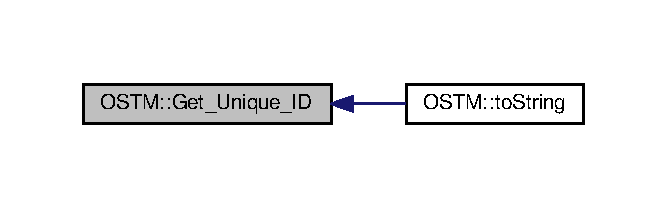
\includegraphics[width=320pt]{class_o_s_t_m_a5a01a8b98d16b1d1904ecf9356e7b71d_icgraph}
\end{center}
\end{figure}


\index{O\+S\+TM@{O\+S\+TM}!Get\+\_\+\+Version@{Get\+\_\+\+Version}}
\index{Get\+\_\+\+Version@{Get\+\_\+\+Version}!O\+S\+TM@{O\+S\+TM}}
\subsubsection[{\texorpdfstring{Get\+\_\+\+Version() const }{Get_Version() const }}]{\setlength{\rightskip}{0pt plus 5cm}int O\+S\+T\+M\+::\+Get\+\_\+\+Version (
\begin{DoxyParamCaption}
{}
\end{DoxyParamCaption}
) const}\hypertarget{class_o_s_t_m_a1f1db9d482f22c8e7caa17dfb340626b}{}\label{class_o_s_t_m_a1f1db9d482f22c8e7caa17dfb340626b}


getter for version number 


\begin{DoxyParams}{Parameters}
{\em version} & int \\
\hline
\end{DoxyParams}


Definition at line 89 of file O\+S\+T\+M.\+cpp.



Here is the caller graph for this function\+:\nopagebreak
\begin{figure}[H]
\begin{center}
\leavevmode
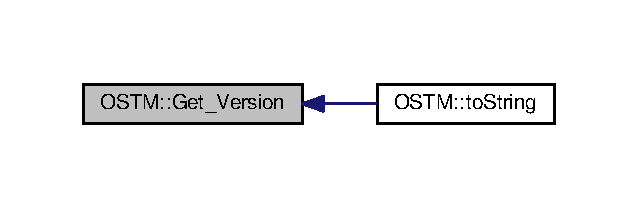
\includegraphics[width=306pt]{class_o_s_t_m_a1f1db9d482f22c8e7caa17dfb340626b_icgraph}
\end{center}
\end{figure}


\index{O\+S\+TM@{O\+S\+TM}!get\+Base\+Copy@{get\+Base\+Copy}}
\index{get\+Base\+Copy@{get\+Base\+Copy}!O\+S\+TM@{O\+S\+TM}}
\subsubsection[{\texorpdfstring{get\+Base\+Copy(std\+::shared\+\_\+ptr$<$ O\+S\+T\+M $>$ object)}{getBaseCopy(std::shared_ptr< OSTM > object)}}]{\setlength{\rightskip}{0pt plus 5cm}virtual std\+::shared\+\_\+ptr$<${\bf O\+S\+TM}$>$ O\+S\+T\+M\+::get\+Base\+Copy (
\begin{DoxyParamCaption}
\item[{std\+::shared\+\_\+ptr$<$ {\bf O\+S\+TM} $>$}]{object}
\end{DoxyParamCaption}
)\hspace{0.3cm}{\ttfamily [inline]}, {\ttfamily [virtual]}}\hypertarget{class_o_s_t_m_a0bfa3763bd441407dd6365f42714f94c}{}\label{class_o_s_t_m_a0bfa3763bd441407dd6365f42714f94c}


\hyperlink{class_o_s_t_m}{O\+S\+TM} required virtual method for returning a pointer that is copy of the original pointer. 



Definition at line 38 of file O\+S\+T\+M.\+h.

\index{O\+S\+TM@{O\+S\+TM}!increase\+\_\+\+Version\+Number@{increase\+\_\+\+Version\+Number}}
\index{increase\+\_\+\+Version\+Number@{increase\+\_\+\+Version\+Number}!O\+S\+TM@{O\+S\+TM}}
\subsubsection[{\texorpdfstring{increase\+\_\+\+Version\+Number()}{increase_VersionNumber()}}]{\setlength{\rightskip}{0pt plus 5cm}void O\+S\+T\+M\+::increase\+\_\+\+Version\+Number (
\begin{DoxyParamCaption}
{}
\end{DoxyParamCaption}
)}\hypertarget{class_o_s_t_m_a5f90caa4384d371c16b7cac860d9f89a}{}\label{class_o_s_t_m_a5f90caa4384d371c16b7cac860d9f89a}


commit time increase version number to child object 


\begin{DoxyParams}{Parameters}
{\em version} & int \\
\hline
\end{DoxyParams}


Definition at line 97 of file O\+S\+T\+M.\+cpp.



Here is the caller graph for this function\+:\nopagebreak
\begin{figure}[H]
\begin{center}
\leavevmode
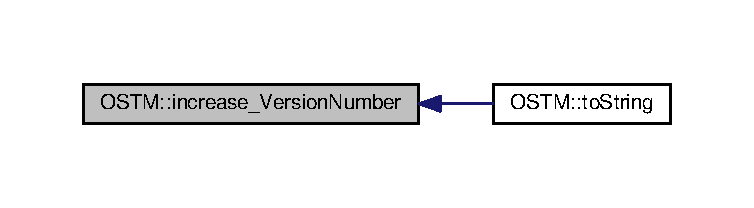
\includegraphics[width=350pt]{class_o_s_t_m_a5f90caa4384d371c16b7cac860d9f89a_icgraph}
\end{center}
\end{figure}


\index{O\+S\+TM@{O\+S\+TM}!Is\+\_\+\+Abort\+\_\+\+Transaction@{Is\+\_\+\+Abort\+\_\+\+Transaction}}
\index{Is\+\_\+\+Abort\+\_\+\+Transaction@{Is\+\_\+\+Abort\+\_\+\+Transaction}!O\+S\+TM@{O\+S\+TM}}
\subsubsection[{\texorpdfstring{Is\+\_\+\+Abort\+\_\+\+Transaction() const }{Is_Abort_Transaction() const }}]{\setlength{\rightskip}{0pt plus 5cm}bool O\+S\+T\+M\+::\+Is\+\_\+\+Abort\+\_\+\+Transaction (
\begin{DoxyParamCaption}
{}
\end{DoxyParamCaption}
) const}\hypertarget{class_o_s_t_m_afc2851abf5342c3c67342c2c14820115}{}\label{class_o_s_t_m_afc2851abf5342c3c67342c2c14820115}


N\+OT U\+S\+ED Y\+ET. 


\begin{DoxyParams}{Parameters}
{\em abort\+\_\+\+Transaction} & boolean \\
\hline
\end{DoxyParams}


Definition at line 126 of file O\+S\+T\+M.\+cpp.



Here is the caller graph for this function\+:\nopagebreak
\begin{figure}[H]
\begin{center}
\leavevmode
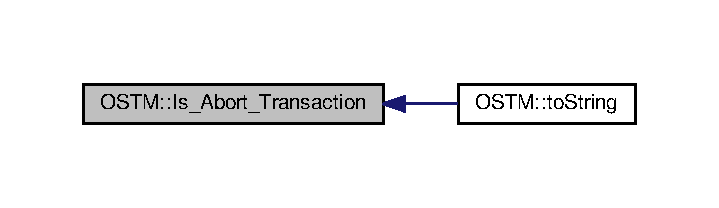
\includegraphics[width=345pt]{class_o_s_t_m_afc2851abf5342c3c67342c2c14820115_icgraph}
\end{center}
\end{figure}


\index{O\+S\+TM@{O\+S\+TM}!Is\+\_\+\+Can\+\_\+\+Commit@{Is\+\_\+\+Can\+\_\+\+Commit}}
\index{Is\+\_\+\+Can\+\_\+\+Commit@{Is\+\_\+\+Can\+\_\+\+Commit}!O\+S\+TM@{O\+S\+TM}}
\subsubsection[{\texorpdfstring{Is\+\_\+\+Can\+\_\+\+Commit() const }{Is_Can_Commit() const }}]{\setlength{\rightskip}{0pt plus 5cm}bool O\+S\+T\+M\+::\+Is\+\_\+\+Can\+\_\+\+Commit (
\begin{DoxyParamCaption}
{}
\end{DoxyParamCaption}
) const}\hypertarget{class_o_s_t_m_a8df39ced3b401aa466df97e26d14b1b7}{}\label{class_o_s_t_m_a8df39ced3b401aa466df97e26d14b1b7}


N\+OT U\+S\+ED Y\+ET. 


\begin{DoxyParams}{Parameters}
{\em can\+Commit} & boolean \\
\hline
\end{DoxyParams}


Definition at line 112 of file O\+S\+T\+M.\+cpp.



Here is the caller graph for this function\+:\nopagebreak
\begin{figure}[H]
\begin{center}
\leavevmode
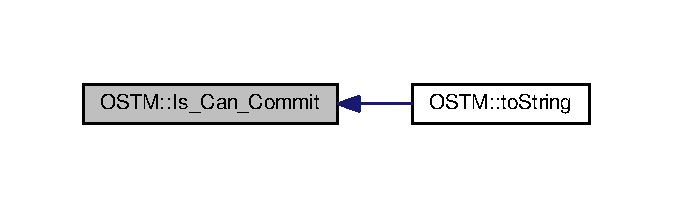
\includegraphics[width=323pt]{class_o_s_t_m_a8df39ced3b401aa466df97e26d14b1b7_icgraph}
\end{center}
\end{figure}


\index{O\+S\+TM@{O\+S\+TM}!is\+\_\+\+Locked@{is\+\_\+\+Locked}}
\index{is\+\_\+\+Locked@{is\+\_\+\+Locked}!O\+S\+TM@{O\+S\+TM}}
\subsubsection[{\texorpdfstring{is\+\_\+\+Locked()}{is_Locked()}}]{\setlength{\rightskip}{0pt plus 5cm}bool O\+S\+T\+M\+::is\+\_\+\+Locked (
\begin{DoxyParamCaption}
{}
\end{DoxyParamCaption}
)}\hypertarget{class_o_s_t_m_afb6520023ed2c4a6188b688c46f192d0}{}\label{class_o_s_t_m_afb6520023ed2c4a6188b688c46f192d0}


object unique lock, try locks mutex return boolean value depends on the lock state 


\begin{DoxyParams}{Parameters}
{\em mutex} & std\+::mutex \\
\hline
\end{DoxyParams}


Definition at line 147 of file O\+S\+T\+M.\+cpp.



Here is the caller graph for this function\+:\nopagebreak
\begin{figure}[H]
\begin{center}
\leavevmode
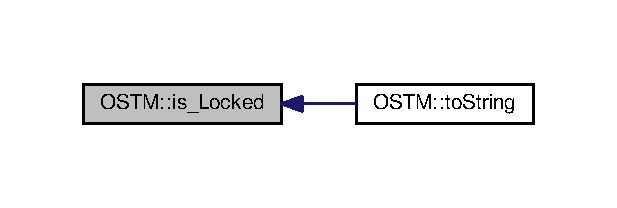
\includegraphics[width=296pt]{class_o_s_t_m_afb6520023ed2c4a6188b688c46f192d0_icgraph}
\end{center}
\end{figure}


\index{O\+S\+TM@{O\+S\+TM}!lock\+\_\+\+Mutex@{lock\+\_\+\+Mutex}}
\index{lock\+\_\+\+Mutex@{lock\+\_\+\+Mutex}!O\+S\+TM@{O\+S\+TM}}
\subsubsection[{\texorpdfstring{lock\+\_\+\+Mutex()}{lock_Mutex()}}]{\setlength{\rightskip}{0pt plus 5cm}void O\+S\+T\+M\+::lock\+\_\+\+Mutex (
\begin{DoxyParamCaption}
{}
\end{DoxyParamCaption}
)}\hypertarget{class_o_s_t_m_af192c598a3c647f37aaba5757e60240f}{}\label{class_o_s_t_m_af192c598a3c647f37aaba5757e60240f}


object unique lock, locks mutex 


\begin{DoxyParams}{Parameters}
{\em mutex} & std\+::mutex \\
\hline
\end{DoxyParams}


Definition at line 133 of file O\+S\+T\+M.\+cpp.



Here is the caller graph for this function\+:\nopagebreak
\begin{figure}[H]
\begin{center}
\leavevmode
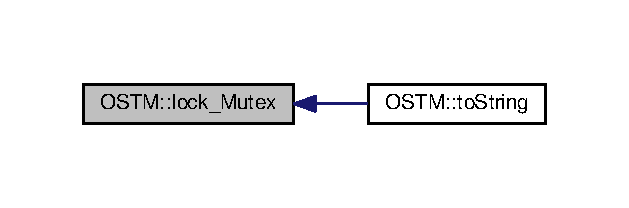
\includegraphics[width=302pt]{class_o_s_t_m_af192c598a3c647f37aaba5757e60240f_icgraph}
\end{center}
\end{figure}


\index{O\+S\+TM@{O\+S\+TM}!Set\+\_\+\+Abort\+\_\+\+Transaction@{Set\+\_\+\+Abort\+\_\+\+Transaction}}
\index{Set\+\_\+\+Abort\+\_\+\+Transaction@{Set\+\_\+\+Abort\+\_\+\+Transaction}!O\+S\+TM@{O\+S\+TM}}
\subsubsection[{\texorpdfstring{Set\+\_\+\+Abort\+\_\+\+Transaction(bool abort\+Transaction)}{Set_Abort_Transaction(bool abortTransaction)}}]{\setlength{\rightskip}{0pt plus 5cm}void O\+S\+T\+M\+::\+Set\+\_\+\+Abort\+\_\+\+Transaction (
\begin{DoxyParamCaption}
\item[{bool}]{abort\+Transaction}
\end{DoxyParamCaption}
)}\hypertarget{class_o_s_t_m_aba384cf65c5f56f5b86833730c3c6ea4}{}\label{class_o_s_t_m_aba384cf65c5f56f5b86833730c3c6ea4}


N\+OT U\+S\+ED Y\+ET. 


\begin{DoxyParams}{Parameters}
{\em abort\+\_\+\+Transaction} & boolean \\
\hline
\end{DoxyParams}


Definition at line 119 of file O\+S\+T\+M.\+cpp.



Here is the caller graph for this function\+:\nopagebreak
\begin{figure}[H]
\begin{center}
\leavevmode
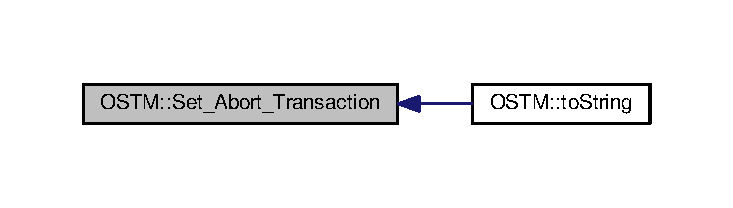
\includegraphics[width=350pt]{class_o_s_t_m_aba384cf65c5f56f5b86833730c3c6ea4_icgraph}
\end{center}
\end{figure}


\index{O\+S\+TM@{O\+S\+TM}!Set\+\_\+\+Can\+\_\+\+Commit@{Set\+\_\+\+Can\+\_\+\+Commit}}
\index{Set\+\_\+\+Can\+\_\+\+Commit@{Set\+\_\+\+Can\+\_\+\+Commit}!O\+S\+TM@{O\+S\+TM}}
\subsubsection[{\texorpdfstring{Set\+\_\+\+Can\+\_\+\+Commit(bool can\+Commit)}{Set_Can_Commit(bool canCommit)}}]{\setlength{\rightskip}{0pt plus 5cm}void O\+S\+T\+M\+::\+Set\+\_\+\+Can\+\_\+\+Commit (
\begin{DoxyParamCaption}
\item[{bool}]{can\+Commit}
\end{DoxyParamCaption}
)}\hypertarget{class_o_s_t_m_a813ee61c9d1c83c6a6ae30d12aca8a5d}{}\label{class_o_s_t_m_a813ee61c9d1c83c6a6ae30d12aca8a5d}


N\+OT U\+S\+ED Y\+ET. 


\begin{DoxyParams}{Parameters}
{\em can\+Commit} & boolean \\
\hline
\end{DoxyParams}


Definition at line 105 of file O\+S\+T\+M.\+cpp.



Here is the caller graph for this function\+:\nopagebreak
\begin{figure}[H]
\begin{center}
\leavevmode
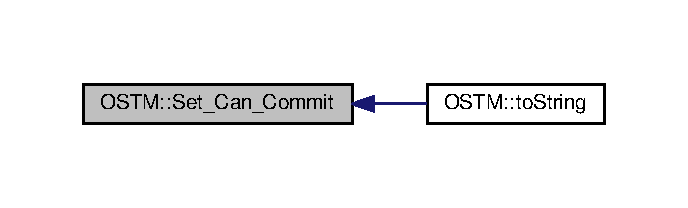
\includegraphics[width=330pt]{class_o_s_t_m_a813ee61c9d1c83c6a6ae30d12aca8a5d_icgraph}
\end{center}
\end{figure}


\index{O\+S\+TM@{O\+S\+TM}!Set\+\_\+\+Unique\+\_\+\+ID@{Set\+\_\+\+Unique\+\_\+\+ID}}
\index{Set\+\_\+\+Unique\+\_\+\+ID@{Set\+\_\+\+Unique\+\_\+\+ID}!O\+S\+TM@{O\+S\+TM}}
\subsubsection[{\texorpdfstring{Set\+\_\+\+Unique\+\_\+\+I\+D(int unique\+I\+D)}{Set_Unique_ID(int uniqueID)}}]{\setlength{\rightskip}{0pt plus 5cm}void O\+S\+T\+M\+::\+Set\+\_\+\+Unique\+\_\+\+ID (
\begin{DoxyParamCaption}
\item[{int}]{unique\+ID}
\end{DoxyParamCaption}
)}\hypertarget{class_o_s_t_m_ab5019a32185631c08abbf826422f2d93}{}\label{class_o_s_t_m_ab5019a32185631c08abbf826422f2d93}


setter for unique id 


\begin{DoxyParams}{Parameters}
{\em unique\+ID} & int \\
\hline
\end{DoxyParams}


Definition at line 66 of file O\+S\+T\+M.\+cpp.



Here is the caller graph for this function\+:\nopagebreak
\begin{figure}[H]
\begin{center}
\leavevmode
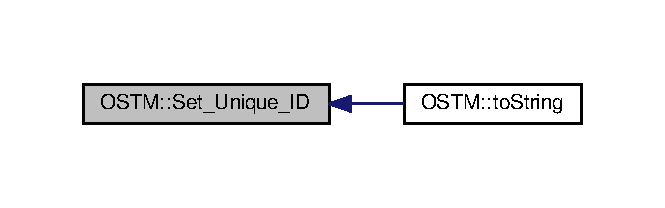
\includegraphics[width=319pt]{class_o_s_t_m_ab5019a32185631c08abbf826422f2d93_icgraph}
\end{center}
\end{figure}


\index{O\+S\+TM@{O\+S\+TM}!Set\+\_\+\+Version@{Set\+\_\+\+Version}}
\index{Set\+\_\+\+Version@{Set\+\_\+\+Version}!O\+S\+TM@{O\+S\+TM}}
\subsubsection[{\texorpdfstring{Set\+\_\+\+Version(int version)}{Set_Version(int version)}}]{\setlength{\rightskip}{0pt plus 5cm}void O\+S\+T\+M\+::\+Set\+\_\+\+Version (
\begin{DoxyParamCaption}
\item[{int}]{version}
\end{DoxyParamCaption}
)}\hypertarget{class_o_s_t_m_a9529ad8d6d28c1f0cc9b86ed91df1ae1}{}\label{class_o_s_t_m_a9529ad8d6d28c1f0cc9b86ed91df1ae1}


setter for version number 


\begin{DoxyParams}{Parameters}
{\em version} & int \\
\hline
\end{DoxyParams}


Definition at line 81 of file O\+S\+T\+M.\+cpp.



Here is the caller graph for this function\+:\nopagebreak
\begin{figure}[H]
\begin{center}
\leavevmode
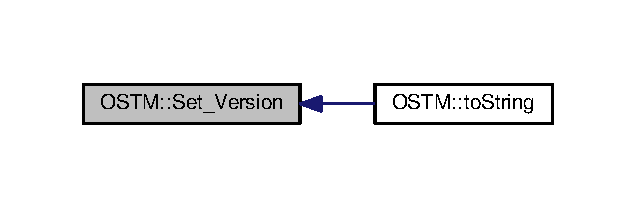
\includegraphics[width=305pt]{class_o_s_t_m_a9529ad8d6d28c1f0cc9b86ed91df1ae1_icgraph}
\end{center}
\end{figure}


\index{O\+S\+TM@{O\+S\+TM}!to\+String@{to\+String}}
\index{to\+String@{to\+String}!O\+S\+TM@{O\+S\+TM}}
\subsubsection[{\texorpdfstring{to\+String()}{toString()}}]{\setlength{\rightskip}{0pt plus 5cm}virtual void O\+S\+T\+M\+::to\+String (
\begin{DoxyParamCaption}
{}
\end{DoxyParamCaption}
)\hspace{0.3cm}{\ttfamily [inline]}, {\ttfamily [virtual]}}\hypertarget{class_o_s_t_m_a513396a115f2987fd07c203309ae8a59}{}\label{class_o_s_t_m_a513396a115f2987fd07c203309ae8a59}


\hyperlink{class_o_s_t_m}{O\+S\+TM} required virtual method for display object. 



Definition at line 42 of file O\+S\+T\+M.\+h.



Here is the call graph for this function\+:\nopagebreak
\begin{figure}[H]
\begin{center}
\leavevmode
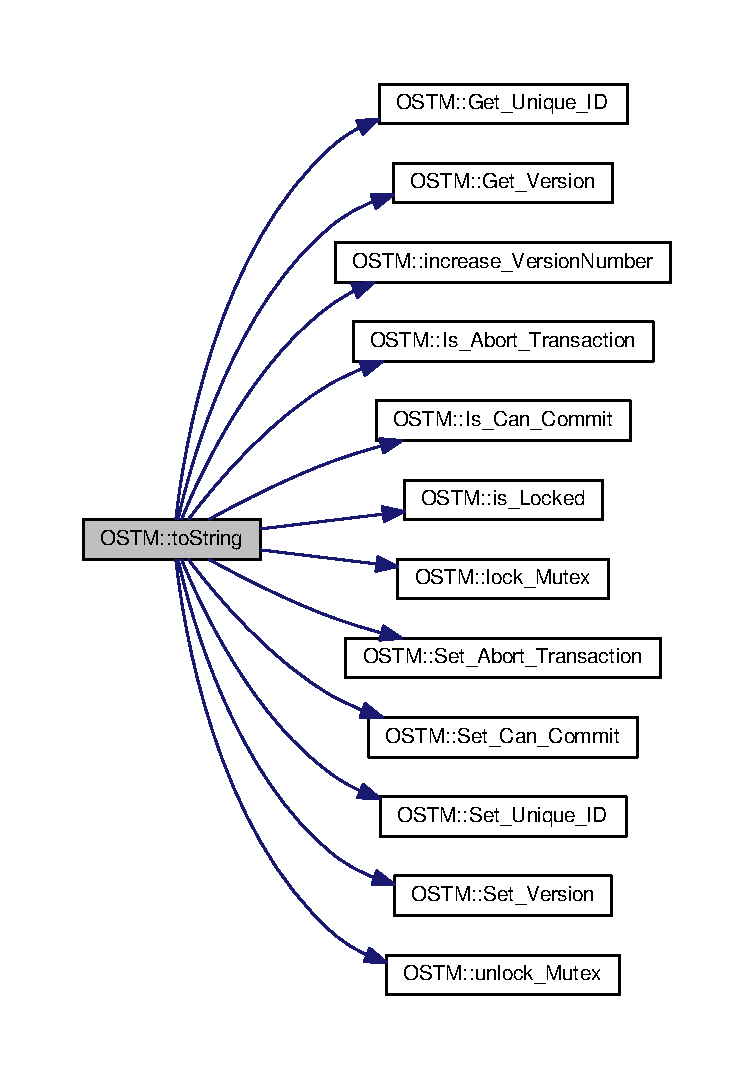
\includegraphics[width=350pt]{class_o_s_t_m_a513396a115f2987fd07c203309ae8a59_cgraph}
\end{center}
\end{figure}


\index{O\+S\+TM@{O\+S\+TM}!unlock\+\_\+\+Mutex@{unlock\+\_\+\+Mutex}}
\index{unlock\+\_\+\+Mutex@{unlock\+\_\+\+Mutex}!O\+S\+TM@{O\+S\+TM}}
\subsubsection[{\texorpdfstring{unlock\+\_\+\+Mutex()}{unlock_Mutex()}}]{\setlength{\rightskip}{0pt plus 5cm}void O\+S\+T\+M\+::unlock\+\_\+\+Mutex (
\begin{DoxyParamCaption}
{}
\end{DoxyParamCaption}
)}\hypertarget{class_o_s_t_m_a6cd703bc26c719fd95b4f5362d050762}{}\label{class_o_s_t_m_a6cd703bc26c719fd95b4f5362d050762}


object unique lock, unlocks mutex 


\begin{DoxyParams}{Parameters}
{\em mutex} & std\+::mutex \\
\hline
\end{DoxyParams}


Definition at line 140 of file O\+S\+T\+M.\+cpp.



Here is the caller graph for this function\+:\nopagebreak
\begin{figure}[H]
\begin{center}
\leavevmode
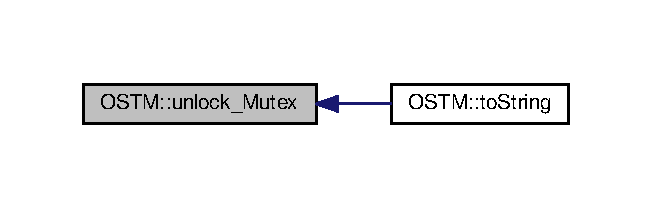
\includegraphics[width=313pt]{class_o_s_t_m_a6cd703bc26c719fd95b4f5362d050762_icgraph}
\end{center}
\end{figure}




The documentation for this class was generated from the following files\+:\begin{DoxyCompactItemize}
\item 
/media/zoltan/\+Data/00\+\_\+2018\+\_\+\+I\+T\+Carlow/00\+\_\+\+Modules/06\+\_\+\+Project/\+Documents/\+Git\+\_\+\+Sync/\+Shared\+\_\+\+O\+\_\+\+S\+T\+M/\hyperlink{_o_s_t_m_8h}{O\+S\+T\+M.\+h}\item 
/media/zoltan/\+Data/00\+\_\+2018\+\_\+\+I\+T\+Carlow/00\+\_\+\+Modules/06\+\_\+\+Project/\+Documents/\+Git\+\_\+\+Sync/\+Shared\+\_\+\+O\+\_\+\+S\+T\+M/\hyperlink{_o_s_t_m_8cpp}{O\+S\+T\+M.\+cpp}\end{DoxyCompactItemize}

\hypertarget{class_t_m}{}\section{TM Class Reference}
\label{class_t_m}\index{TM@{TM}}


{\ttfamily \#include $<$T\+M.\+h$>$}

\subsection*{Public Member Functions}
\begin{DoxyCompactItemize}
\item 
std\+::shared\+\_\+ptr$<$ \hyperlink{class_t_x}{TX} $>$ const \hyperlink{class_t_m_a41cb0226cc4080c931651b13f74a0075}{\+\_\+get\+\_\+tx} ()
\begin{DoxyCompactList}\small\item\em \+\_\+get\+\_\+tx std\+::shared\+\_\+ptr$<$\+T\+X$>$, returning a shared pointer with the transaction \end{DoxyCompactList}\item 
void \hyperlink{class_t_m_a5e2d1127f2429f2f524d25f430eade06}{\+\_\+\+T\+X\+\_\+\+E\+X\+IT} ()
\begin{DoxyCompactList}\small\item\em \+\_\+\+T\+X\+\_\+\+E\+X\+IT void, the thread calls the ostm\+\_\+exit function in the transaction, and clear all elements from the shared global collection associated with the main process \end{DoxyCompactList}\item 
void \hyperlink{class_t_m_a1d6891b1d3e71cc0acef54e7afe71c09}{print\+\_\+all} ()
\begin{DoxyCompactList}\small\item\em O\+N\+LY F\+OR T\+E\+S\+T\+I\+NG print\+\_\+all void, print out all object key from tx\+M\+AP collection. \end{DoxyCompactList}\end{DoxyCompactItemize}
\subsection*{Static Public Member Functions}
\begin{DoxyCompactItemize}
\item 
static \hyperlink{class_t_m}{TM} \& \hyperlink{class_t_m_a7ce5f35e0dae76df4fe116cf905bbe60}{Instance} ()
\begin{DoxyCompactList}\small\item\em Scott Meyer\textquotesingle{}s Singleton creation, what is thread safe. \end{DoxyCompactList}\end{DoxyCompactItemize}


\subsection{Detailed Description}


Definition at line 58 of file T\+M.\+h.



\subsection{Member Function Documentation}
\index{TM@{TM}!\+\_\+get\+\_\+tx@{\+\_\+get\+\_\+tx}}
\index{\+\_\+get\+\_\+tx@{\+\_\+get\+\_\+tx}!TM@{TM}}
\subsubsection[{\texorpdfstring{\+\_\+get\+\_\+tx()}{_get_tx()}}]{\setlength{\rightskip}{0pt plus 5cm}std\+::shared\+\_\+ptr$<$ {\bf TX} $>$ const T\+M\+::\+\_\+get\+\_\+tx (
\begin{DoxyParamCaption}
{}
\end{DoxyParamCaption}
)}\hypertarget{class_t_m_a41cb0226cc4080c931651b13f74a0075}{}\label{class_t_m_a41cb0226cc4080c931651b13f74a0075}


\+\_\+get\+\_\+tx std\+::shared\+\_\+ptr$<$\+T\+X$>$, returning a shared pointer with the transaction 

\+\_\+get\+\_\+tx std\+::shared\+\_\+ptr$<$\+T\+X$>$, return a shared\+\_\+ptr with the Transaction object, if \hyperlink{class_t_x}{TX} not exists then create one, else increasing the nesting level  std\+::mutex, protect shared collection from critical section


\begin{DoxyParams}{Parameters}
{\em guard} & std\+::lock\+\_\+guard, locks the register\+\_\+\+Lock mutex, unlock automatically when goes out of the scope \\
\hline
\end{DoxyParams}


Definition at line 78 of file T\+M.\+cpp.



Here is the caller graph for this function\+:
% FIG 0


\index{TM@{TM}!\+\_\+\+T\+X\+\_\+\+E\+X\+IT@{\+\_\+\+T\+X\+\_\+\+E\+X\+IT}}
\index{\+\_\+\+T\+X\+\_\+\+E\+X\+IT@{\+\_\+\+T\+X\+\_\+\+E\+X\+IT}!TM@{TM}}
\subsubsection[{\texorpdfstring{\+\_\+\+T\+X\+\_\+\+E\+X\+I\+T()}{_TX_EXIT()}}]{\setlength{\rightskip}{0pt plus 5cm}void T\+M\+::\+\_\+\+T\+X\+\_\+\+E\+X\+IT (
\begin{DoxyParamCaption}
{}
\end{DoxyParamCaption}
)}\hypertarget{class_t_m_a5e2d1127f2429f2f524d25f430eade06}{}\label{class_t_m_a5e2d1127f2429f2f524d25f430eade06}


\+\_\+\+T\+X\+\_\+\+E\+X\+IT void, the thread calls the ostm\+\_\+exit function in the transaction, and clear all elements from the shared global collection associated with the main process 

\+\_\+\+T\+X\+\_\+\+E\+X\+IT void, the thread calls the ostm\+\_\+exit function in the transaction, and clear all elements from the shared global collection associated with the main process  tx \hyperlink{class_t_x}{TX}, local object to function in transaction 

Definition at line 101 of file T\+M.\+cpp.



Here is the call graph for this function\+:
% FIG 1




Here is the caller graph for this function\+:
% FIG 2


\index{TM@{TM}!Instance@{Instance}}
\index{Instance@{Instance}!TM@{TM}}
\subsubsection[{\texorpdfstring{Instance()}{Instance()}}]{\setlength{\rightskip}{0pt plus 5cm}{\bf TM} \& T\+M\+::\+Instance (
\begin{DoxyParamCaption}
{}
\end{DoxyParamCaption}
)\hspace{0.3cm}{\ttfamily [static]}}\hypertarget{class_t_m_a7ce5f35e0dae76df4fe116cf905bbe60}{}\label{class_t_m_a7ce5f35e0dae76df4fe116cf905bbe60}


Scott Meyer\textquotesingle{}s Singleton creation, what is thread safe. 

Instance \hyperlink{class_t_m}{TM}, return the same singleton object to any process.


\begin{DoxyParams}{Parameters}
{\em \+\_\+instance} & \hyperlink{class_t_m}{TM}, static class reference to the instance of the Transaction Manager class \\
\hline
{\em \+\_\+instance} & ppid, assigning the process id whoever created the Singleton instance \\
\hline
\end{DoxyParams}


Definition at line 28 of file T\+M.\+cpp.



Here is the caller graph for this function\+:
% FIG 3


\index{TM@{TM}!print\+\_\+all@{print\+\_\+all}}
\index{print\+\_\+all@{print\+\_\+all}!TM@{TM}}
\subsubsection[{\texorpdfstring{print\+\_\+all()}{print_all()}}]{\setlength{\rightskip}{0pt plus 5cm}void T\+M\+::print\+\_\+all (
\begin{DoxyParamCaption}
{}
\end{DoxyParamCaption}
)}\hypertarget{class_t_m_a1d6891b1d3e71cc0acef54e7afe71c09}{}\label{class_t_m_a1d6891b1d3e71cc0acef54e7afe71c09}


O\+N\+LY F\+OR T\+E\+S\+T\+I\+NG print\+\_\+all void, print out all object key from tx\+M\+AP collection. 

O\+N\+LY F\+OR T\+E\+S\+T\+I\+NG print\+\_\+all void, prints all object in the tx\+Map 

Definition at line 121 of file T\+M.\+cpp.



Here is the caller graph for this function\+:
% FIG 4




The documentation for this class was generated from the following files\+:\begin{DoxyCompactItemize}
\item 
\hyperlink{_t_m_8h}{T\+M.\+h}\item 
\hyperlink{_t_m_8cpp}{T\+M.\+cpp}\end{DoxyCompactItemize}

\hypertarget{class_t_x}{}\subsection{TX Class Reference}
\label{class_t_x}\index{TX@{TX}}


Collaboration diagram for TX\+:\nopagebreak
\begin{figure}[H]
\begin{center}
\leavevmode
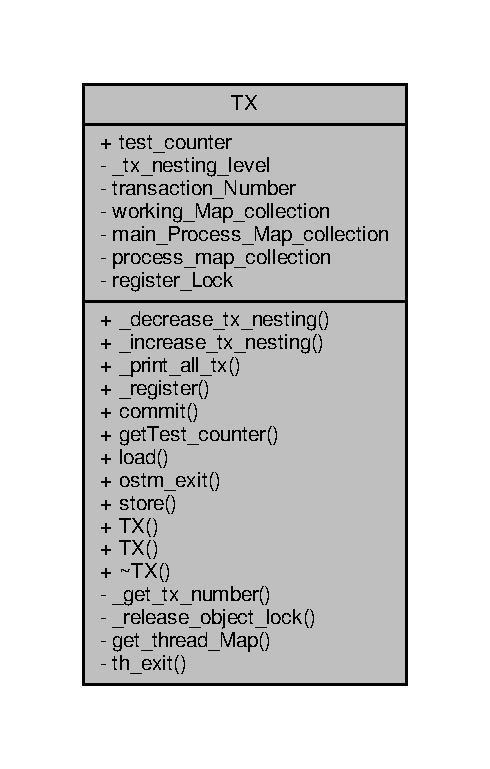
\includegraphics[width=207pt]{class_t_x__coll__graph}
\end{center}
\end{figure}
\subsubsection*{Public Member Functions}
\begin{DoxyCompactItemize}
\item 
\hyperlink{class_t_x_a8a4b83eab0171ae834bfa92bbced1094}{TX} (std\+::thread\+::id id)
\begin{DoxyCompactList}\small\item\em Constructor. \end{DoxyCompactList}\item 
\hyperlink{class_t_x_abecf854cc3228ab6dd51175b3cd1c70a}{$\sim$\+TX} ()\hypertarget{class_t_x_abecf854cc3228ab6dd51175b3cd1c70a}{}\label{class_t_x_abecf854cc3228ab6dd51175b3cd1c70a}

\begin{DoxyCompactList}\small\item\em De-\/constructor. \end{DoxyCompactList}\item 
\hyperlink{class_t_x_ab96b3dd2bfd621b47307f0af3ec4f35c}{TX} (const \hyperlink{class_t_x}{TX} \&orig)\hypertarget{class_t_x_ab96b3dd2bfd621b47307f0af3ec4f35c}{}\label{class_t_x_ab96b3dd2bfd621b47307f0af3ec4f35c}

\begin{DoxyCompactList}\small\item\em Default copy constructor. \end{DoxyCompactList}\item 
void \hyperlink{class_t_x_aa9739c5c2077454c779098db7baefc2b}{ostm\+\_\+exit} ()
\begin{DoxyCompactList}\small\item\em Delete all map entries associated with the main process. \end{DoxyCompactList}\item 
void \hyperlink{class_t_x_abc32af2f51df97ac483e5bfe7db6ca6e}{\+\_\+register} (std\+::shared\+\_\+ptr$<$ \hyperlink{class_o_s_t_m}{O\+S\+TM} $>$ object)
\begin{DoxyCompactList}\small\item\em Register \hyperlink{class_o_s_t_m}{O\+S\+TM} pointer into S\+TM library. \end{DoxyCompactList}\item 
std\+::shared\+\_\+ptr$<$ \hyperlink{class_o_s_t_m}{O\+S\+TM} $>$ \hyperlink{class_t_x_a1d78262b8831ddd042ed491f2e600e24}{load} (std\+::shared\+\_\+ptr$<$ \hyperlink{class_o_s_t_m}{O\+S\+TM} $>$ object)
\begin{DoxyCompactList}\small\item\em load std\+::shared\+\_\+ptr$<$\+O\+S\+T\+M$>$, returning an std\+::shared\+\_\+ptr$<$\+O\+S\+T\+M$>$ copy of the original pointer, to work with during transaction life time \end{DoxyCompactList}\item 
void \hyperlink{class_t_x_a7dbcb369aa4a3370b6c6829d278ece5d}{store} (std\+::shared\+\_\+ptr$<$ \hyperlink{class_o_s_t_m}{O\+S\+TM} $>$ object)
\begin{DoxyCompactList}\small\item\em Store transactional changes. \end{DoxyCompactList}\item 
bool \hyperlink{class_t_x_a9dde5d356b35e557448e58d260087356}{commit} ()
\begin{DoxyCompactList}\small\item\em Commit transactional changes. \end{DoxyCompactList}\item 
void \hyperlink{class_t_x_a1384bdf12d795854b5d32e7f61ffbdb8}{\+\_\+increase\+\_\+tx\+\_\+nesting} ()
\begin{DoxyCompactList}\small\item\em Add \hyperlink{class_t_x}{TX} nesting level by one. \end{DoxyCompactList}\item 
void \hyperlink{class_t_x_aa3ac499f576326588628ade96b27b4b1}{\+\_\+decrease\+\_\+tx\+\_\+nesting} ()
\begin{DoxyCompactList}\small\item\em Remove \hyperlink{class_t_x}{TX} nesting level by one. \end{DoxyCompactList}\item 
int \hyperlink{class_t_x_ae9bf97930c4670f59d334b345353a71e}{get\+Test\+\_\+counter} ()\hypertarget{class_t_x_ae9bf97930c4670f59d334b345353a71e}{}\label{class_t_x_ae9bf97930c4670f59d334b345353a71e}

\begin{DoxyCompactList}\small\item\em get\+Test\+\_\+counter T\+E\+S\+T\+I\+NG O\+N\+L\+Y!!! returning the value of the test\+\_\+counter stored, number of rollbacks \end{DoxyCompactList}\item 
void \hyperlink{class_t_x_a3d96ed91eb9ec73e16589f705661c5a7}{\+\_\+print\+\_\+all\+\_\+tx} ()
\end{DoxyCompactItemize}
\subsubsection*{Static Public Attributes}
\begin{DoxyCompactItemize}
\item 
static int \hyperlink{class_t_x_a25838234aab99ae891a90eb8623a8b3c}{test\+\_\+counter} = 0
\end{DoxyCompactItemize}
\subsubsection*{Friends}
\begin{DoxyCompactItemize}
\item 
class \hyperlink{class_t_x_adf1ccda799ef5c419cb43b8ae55eb45c}{TM}
\end{DoxyCompactItemize}


\subsubsection{Detailed Description}


Definition at line \hyperlink{_t_x_8h_source_l00024}{24} of file \hyperlink{_t_x_8h_source}{T\+X.\+h}.



\subsubsection{Constructor \& Destructor Documentation}
\index{TX@{TX}!TX@{TX}}
\index{TX@{TX}!TX@{TX}}
\paragraph[{\texorpdfstring{T\+X(std\+::thread\+::id id)}{TX(std::thread::id id)}}]{\setlength{\rightskip}{0pt plus 5cm}T\+X\+::\+TX (
\begin{DoxyParamCaption}
\item[{std\+::thread\+::id}]{id}
\end{DoxyParamCaption}
)}\hypertarget{class_t_x_a8a4b83eab0171ae834bfa92bbced1094}{}\label{class_t_x_a8a4b83eab0171ae834bfa92bbced1094}


Constructor. 


\begin{DoxyParams}{Parameters}
{\em transaction\+\_\+\+Number} & int, to store associated thread \\
\hline
{\em \+\_\+tx\+\_\+nesting\+\_\+level} & int, to store and indicate nesting level of transactions within transaction \\
\hline
\end{DoxyParams}


Definition at line \hyperlink{_t_x_8cpp_source_l00031}{31} of file \hyperlink{_t_x_8cpp_source}{T\+X.\+cpp}.


\begin{DoxyCode}
00031                      \{
00032     this->transaction\_Number = id;
00033     this->\_tx\_nesting\_level = 0;
00034 \}
\end{DoxyCode}


\subsubsection{Member Function Documentation}
\index{TX@{TX}!\+\_\+decrease\+\_\+tx\+\_\+nesting@{\+\_\+decrease\+\_\+tx\+\_\+nesting}}
\index{\+\_\+decrease\+\_\+tx\+\_\+nesting@{\+\_\+decrease\+\_\+tx\+\_\+nesting}!TX@{TX}}
\paragraph[{\texorpdfstring{\+\_\+decrease\+\_\+tx\+\_\+nesting()}{_decrease_tx_nesting()}}]{\setlength{\rightskip}{0pt plus 5cm}void T\+X\+::\+\_\+decrease\+\_\+tx\+\_\+nesting (
\begin{DoxyParamCaption}
{}
\end{DoxyParamCaption}
)}\hypertarget{class_t_x_aa3ac499f576326588628ade96b27b4b1}{}\label{class_t_x_aa3ac499f576326588628ade96b27b4b1}


Remove \hyperlink{class_t_x}{TX} nesting level by one. 

\+\_\+decrease\+\_\+tx\+\_\+nesting decrease the value stored in \+\_\+tx\+\_\+nesting\+\_\+level by one, when outer transactions commiting


\begin{DoxyParams}{Parameters}
{\em \+\_\+tx\+\_\+nesting\+\_\+level} & int \\
\hline
\end{DoxyParams}


Definition at line \hyperlink{_t_x_8cpp_source_l00316}{316} of file \hyperlink{_t_x_8cpp_source}{T\+X.\+cpp}.



Referenced by \hyperlink{_t_x_8cpp_source_l00202}{commit()}.


\begin{DoxyCode}
00316                               \{
00317    \textcolor{comment}{// std::cout << "[this->\_tx\_nesting\_level] = " << this->\_tx\_nesting\_level << std::endl;}
00318     this->\_tx\_nesting\_level -= 1;
00319 ;
00320 \}
\end{DoxyCode}


Here is the caller graph for this function\+:\nopagebreak
\begin{figure}[H]
\begin{center}
\leavevmode
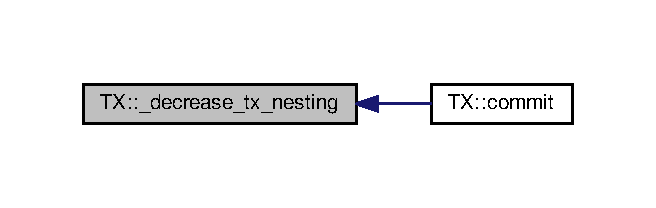
\includegraphics[width=315pt]{class_t_x_aa3ac499f576326588628ade96b27b4b1_icgraph}
\end{center}
\end{figure}


\index{TX@{TX}!\+\_\+increase\+\_\+tx\+\_\+nesting@{\+\_\+increase\+\_\+tx\+\_\+nesting}}
\index{\+\_\+increase\+\_\+tx\+\_\+nesting@{\+\_\+increase\+\_\+tx\+\_\+nesting}!TX@{TX}}
\paragraph[{\texorpdfstring{\+\_\+increase\+\_\+tx\+\_\+nesting()}{_increase_tx_nesting()}}]{\setlength{\rightskip}{0pt plus 5cm}void T\+X\+::\+\_\+increase\+\_\+tx\+\_\+nesting (
\begin{DoxyParamCaption}
{}
\end{DoxyParamCaption}
)}\hypertarget{class_t_x_a1384bdf12d795854b5d32e7f61ffbdb8}{}\label{class_t_x_a1384bdf12d795854b5d32e7f61ffbdb8}


Add \hyperlink{class_t_x}{TX} nesting level by one. 

\+\_\+increase\+\_\+tx\+\_\+nesting increase the value stored in \+\_\+tx\+\_\+nesting\+\_\+level by one, indicate that the transaction nested


\begin{DoxyParams}{Parameters}
{\em \+\_\+tx\+\_\+nesting\+\_\+level} & int \\
\hline
\end{DoxyParams}


Definition at line \hyperlink{_t_x_8cpp_source_l00307}{307} of file \hyperlink{_t_x_8cpp_source}{T\+X.\+cpp}.


\begin{DoxyCode}
00307                               \{
00308       
00309     this->\_tx\_nesting\_level += 1;
00310     \textcolor{comment}{// std::cout << "[this->\_tx\_nesting\_level] = " << this->\_tx\_nesting\_level << std::endl;}
00311 \}
\end{DoxyCode}
\index{TX@{TX}!\+\_\+print\+\_\+all\+\_\+tx@{\+\_\+print\+\_\+all\+\_\+tx}}
\index{\+\_\+print\+\_\+all\+\_\+tx@{\+\_\+print\+\_\+all\+\_\+tx}!TX@{TX}}
\paragraph[{\texorpdfstring{\+\_\+print\+\_\+all\+\_\+tx()}{_print_all_tx()}}]{\setlength{\rightskip}{0pt plus 5cm}void T\+X\+::\+\_\+print\+\_\+all\+\_\+tx (
\begin{DoxyParamCaption}
{}
\end{DoxyParamCaption}
)}\hypertarget{class_t_x_a3d96ed91eb9ec73e16589f705661c5a7}{}\label{class_t_x_a3d96ed91eb9ec73e16589f705661c5a7}
O\+N\+LY F\+OR T\+E\+S\+T\+I\+NG C\+H\+E\+CK T\+HE M\+AP A\+F\+T\+ER T\+H\+R\+E\+AD E\+X\+IT A\+ND A\+LL S\+H\+O\+U\+LD BE D\+E\+L\+E\+T\+E\+D!!!!!!! 

Definition at line \hyperlink{_t_x_8cpp_source_l00346}{346} of file \hyperlink{_t_x_8cpp_source}{T\+X.\+cpp}.


\begin{DoxyCode}
00346                        \{
00347 
00348     std::cout << \textcolor{stringliteral}{"[PRINTALLTHREAD]"} << std::endl;
00349     std::map< int, std::shared\_ptr<OSTM> >::iterator it;
00350     \textcolor{comment}{/*}
00351 \textcolor{comment}{     * All registered thread id in the TX global 
}
00352 \textcolor{comment}{     */}
00353      pid\_t ppid = getppid();
00354     std::map<pid\_t, std::map< int, int >>::iterator process\_map\_collection\_Iterator = 
      TX::process\_map\_collection.find(ppid);
00355     \textcolor{keywordflow}{if} (process\_map\_collection\_Iterator != TX::process\_map\_collection.end()) \{
00356 
00357         \textcolor{keywordflow}{for} (\textcolor{keyword}{auto} current = process\_map\_collection\_Iterator->second.begin(); current != 
      process\_map\_collection\_Iterator->second.end(); ++current) \{
00358             it = working\_Map\_collection.find(current->first);
00359             \textcolor{keywordflow}{if}(it != working\_Map\_collection.end())\{
00360                 std::cout << \textcolor{stringliteral}{"[Unique number ] : "} <<it->second->Get\_Unique\_ID() << std::endl;
00361             \}
00362 
00363             
00364         \}
00365      
00366     \}
00367 \}\end{DoxyCode}
\index{TX@{TX}!\+\_\+register@{\+\_\+register}}
\index{\+\_\+register@{\+\_\+register}!TX@{TX}}
\paragraph[{\texorpdfstring{\+\_\+register(std\+::shared\+\_\+ptr$<$ O\+S\+T\+M $>$ object)}{_register(std::shared_ptr< OSTM > object)}}]{\setlength{\rightskip}{0pt plus 5cm}void T\+X\+::\+\_\+register (
\begin{DoxyParamCaption}
\item[{std\+::shared\+\_\+ptr$<$ {\bf O\+S\+TM} $>$}]{object}
\end{DoxyParamCaption}
)}\hypertarget{class_t_x_abc32af2f51df97ac483e5bfe7db6ca6e}{}\label{class_t_x_abc32af2f51df97ac483e5bfe7db6ca6e}


Register \hyperlink{class_o_s_t_m}{O\+S\+TM} pointer into S\+TM library. 

register void, receives an std\+::shared\+\_\+ptr$<$\+O\+S\+T\+M$>$ that point to the original memory space to protect from reca conditions


\begin{DoxyParams}{Parameters}
{\em working\+\_\+\+Map\+\_\+collection} & std\+::map, store all the std\+::shared\+\_\+ptr$<$\+O\+S\+T\+M$>$ pointer in the transaction \\
\hline
{\em main\+\_\+\+Process\+\_\+\+Map\+\_\+collection} & std\+::map, store all std\+::shared\+\_\+ptr$<$\+O\+S\+T\+M$>$ from all transaction, used to lock and compare the objects \\
\hline
{\em process\+\_\+map\+\_\+collection} & std\+::map, store all std\+::shared\+\_\+ptr$<$\+O\+S\+T\+M$>$ unique ID from all transaction, used to delete all pointers used by the main process, from all transaction before the program exit. \\
\hline
{\em std\+::lock\+\_\+guard} & use register\+\_\+\+Lock(mutex) shared lock between all transaction \\
\hline
{\em ppid} & int, store main process number \\
\hline
\end{DoxyParams}


Definition at line \hyperlink{_t_x_8cpp_source_l00104}{104} of file \hyperlink{_t_x_8cpp_source}{T\+X.\+cpp}.


\begin{DoxyCode}
00104                                              \{
00105     \textcolor{comment}{/*}
00106 \textcolor{comment}{     * MUST USE SHARED LOCK TO PROTECT SHARED GLOBAL MAP/COLLECTION 
}
00107 \textcolor{comment}{     */}
00108     std::lock\_guard<std::mutex> guard(TX::register\_Lock);
00109     
00110     \textcolor{comment}{/*}
00111 \textcolor{comment}{     * Check for null pointer !
}
00112 \textcolor{comment}{     * Null pointer can cause segmentation fault!!!
}
00113 \textcolor{comment}{     */}
00114     \textcolor{keywordflow}{if}(\textcolor{keywordtype}{object} == \textcolor{keyword}{nullptr})\{
00115         \textcolor{keywordflow}{throw} std::runtime\_error(std::string(\textcolor{stringliteral}{"[RUNTIME ERROR : NULL POINTER IN REGISTER FUNCTION]"}) );
00116     \}
00117     
00118     pid\_t ppid = getppid();
00119     std::map<pid\_t, std::map< int, int >>::iterator process\_map\_collection\_Iterator = 
      TX::process\_map\_collection.find(ppid);
00120     \textcolor{keywordflow}{if} (process\_map\_collection\_Iterator == TX::process\_map\_collection.end()) \{
00121         \textcolor{comment}{/*}
00122 \textcolor{comment}{         * Register main process/application to the global map
}
00123 \textcolor{comment}{         */}
00124         std::map< int, int >map =  get\_thread\_Map();
00125         TX::process\_map\_collection.insert(\{ppid, map\});
00126         \textcolor{comment}{/*}
00127 \textcolor{comment}{         * Get the map if registered first time
}
00128 \textcolor{comment}{         */}
00129         process\_map\_collection\_Iterator = TX::process\_map\_collection.find(ppid);
00130     \}
00131     std::map<int, std::shared\_ptr<OSTM>>::iterator main\_Process\_Map\_collection\_Iterator = 
      TX::main\_Process\_Map\_collection.find(object->Get\_Unique\_ID());
00132     \textcolor{keywordflow}{if} (main\_Process\_Map\_collection\_Iterator == TX::main\_Process\_Map\_collection.end()) \{
00133         \textcolor{comment}{/*}
00134 \textcolor{comment}{         * Insert to the GLOBAL MAP 
}
00135 \textcolor{comment}{         */}
00136         TX::main\_Process\_Map\_collection.insert(\{\textcolor{keywordtype}{object}->Get\_Unique\_ID(), \textcolor{keywordtype}{object}\});
00137         \textcolor{comment}{/*}
00138 \textcolor{comment}{         * Insert to the GLOBAL MAP as a helper to clean up at end of main process 
}
00139 \textcolor{comment}{         */}
00140         process\_map\_collection\_Iterator->second.insert(\{\textcolor{keywordtype}{object}->Get\_Unique\_ID(), 1\});
00141     \} 
00142 
00143 
00144     std::map< int, std::shared\_ptr<OSTM> >::iterator working\_Map\_collection\_Object\_Shared\_Pointer\_Iterator 
      = working\_Map\_collection.find(object->Get\_Unique\_ID());
00145     \textcolor{keywordflow}{if} (working\_Map\_collection\_Object\_Shared\_Pointer\_Iterator == working\_Map\_collection.end()) \{
00146 
00147         working\_Map\_collection.insert(\{\textcolor{keywordtype}{object}->Get\_Unique\_ID(), \textcolor{keywordtype}{object}->getBaseCopy(\textcolor{keywordtype}{object})\});
00148     \}
00149 
00150 \}
\end{DoxyCode}
\index{TX@{TX}!commit@{commit}}
\index{commit@{commit}!TX@{TX}}
\paragraph[{\texorpdfstring{commit()}{commit()}}]{\setlength{\rightskip}{0pt plus 5cm}bool T\+X\+::commit (
\begin{DoxyParamCaption}
{}
\end{DoxyParamCaption}
)}\hypertarget{class_t_x_a9dde5d356b35e557448e58d260087356}{}\label{class_t_x_a9dde5d356b35e557448e58d260087356}


Commit transactional changes. 

commit bool, returns boolean value T\+R\+U\+E/\+F\+A\+L\+SE depends on the action taken within the function


\begin{DoxyParams}{Parameters}
{\em working\+\_\+\+Map\+\_\+collection} & std\+::map, store all the std\+::shared\+\_\+ptr$<$\+O\+S\+T\+M$>$ pointer in the transaction \\
\hline
{\em main\+\_\+\+Process\+\_\+\+Map\+\_\+collection} & std\+::map, store all std\+::shared\+\_\+ptr$<$\+O\+S\+T\+M$>$ from all transaction, used to lock and compare the objects \\
\hline
{\em can\+\_\+\+Commit} & bool, helps to make decision that the transaction can commit or rollback \\
\hline
\end{DoxyParams}


Definition at line \hyperlink{_t_x_8cpp_source_l00202}{202} of file \hyperlink{_t_x_8cpp_source}{T\+X.\+cpp}.



References \hyperlink{_t_x_8cpp_source_l00316}{\+\_\+decrease\+\_\+tx\+\_\+nesting()}, and \hyperlink{_t_x_8h_source_l00078}{test\+\_\+counter}.


\begin{DoxyCode}
00202                 \{
00203 
00204     \textcolor{keywordtype}{bool} can\_Commit = \textcolor{keyword}{true};
00205  
00206     \textcolor{comment}{/*}
00207 \textcolor{comment}{     * Dealing with nested transactions first 
}
00208 \textcolor{comment}{     */}
00209     \textcolor{keywordflow}{if} (this->\_tx\_nesting\_level > 0) \{
00210         \hyperlink{class_t_x_aa3ac499f576326588628ade96b27b4b1}{\_decrease\_tx\_nesting}();
00211         \textcolor{keywordflow}{return} \textcolor{keyword}{true};
00212     \} 
00213     
00214     std::map< int, std::shared\_ptr<OSTM> >::iterator working\_Map\_collection\_Object\_Shared\_Pointer\_Iterator;
00215 
00216     std::map<int, std::shared\_ptr<OSTM>>::iterator main\_Process\_Map\_collection\_Iterator;
00217     \textcolor{keywordflow}{for} (working\_Map\_collection\_Object\_Shared\_Pointer\_Iterator = working\_Map\_collection.begin(); 
      working\_Map\_collection\_Object\_Shared\_Pointer\_Iterator != working\_Map\_collection.end(); 
      working\_Map\_collection\_Object\_Shared\_Pointer\_Iterator++) \{
00218 
00219             main\_Process\_Map\_collection\_Iterator = TX::main\_Process\_Map\_collection.find(
      working\_Map\_collection\_Object\_Shared\_Pointer\_Iterator->second->Get\_Unique\_ID());
00220             \textcolor{comment}{/*}
00221 \textcolor{comment}{             * Throws runtime error if object can not find
}
00222 \textcolor{comment}{             */}
00223             \textcolor{keywordflow}{if}(main\_Process\_Map\_collection\_Iterator == TX::main\_Process\_Map\_collection.end())
00224             \{
00225                 \textcolor{keywordflow}{throw} std::runtime\_error(std::string(\textcolor{stringliteral}{"[RUNTIME ERROR : CAN'T FIND OBJECT COMMIT FUNCTION]"})
      );
00226             \}
00227 
00228         \textcolor{comment}{/*}
00229 \textcolor{comment}{         * Busy wait WHILE object locked by other thread
}
00230 \textcolor{comment}{         */}
00231         \textcolor{keywordflow}{while}(!(main\_Process\_Map\_collection\_Iterator->second)->is\_Locked());
00232 
00233         \textcolor{keywordflow}{if} (main\_Process\_Map\_collection\_Iterator->second->Get\_Version() > 
      working\_Map\_collection\_Object\_Shared\_Pointer\_Iterator->second->Get\_Version()) \{
00234 
00235             working\_Map\_collection\_Object\_Shared\_Pointer\_Iterator->second->Set\_Can\_Commit(\textcolor{keyword}{false});
00236             can\_Commit = \textcolor{keyword}{false};
00237             \textcolor{keywordflow}{break};
00238         \} \textcolor{keywordflow}{else} \{
00239 
00240             working\_Map\_collection\_Object\_Shared\_Pointer\_Iterator->second->Set\_Can\_Commit(\textcolor{keyword}{true});
00241         \}
00242     \}
00243     \textcolor{keywordflow}{if} (!can\_Commit) \{
00244         \hyperlink{class_t_x_a25838234aab99ae891a90eb8623a8b3c}{TX::test\_counter} += 1;
00245         \textcolor{keywordflow}{for} (working\_Map\_collection\_Object\_Shared\_Pointer\_Iterator = working\_Map\_collection.begin(); 
      working\_Map\_collection\_Object\_Shared\_Pointer\_Iterator != working\_Map\_collection.end(); 
      working\_Map\_collection\_Object\_Shared\_Pointer\_Iterator++) \{
00246           
00247             main\_Process\_Map\_collection\_Iterator  = TX::main\_Process\_Map\_collection.find(
      working\_Map\_collection\_Object\_Shared\_Pointer\_Iterator->second->Get\_Unique\_ID());
00248             (working\_Map\_collection\_Object\_Shared\_Pointer\_Iterator->second)->copy(
      working\_Map\_collection\_Object\_Shared\_Pointer\_Iterator->second, main\_Process\_Map\_collection\_Iterator->second);
00249 
00250         \}
00251         
00252         \_release\_object\_lock();
00253 
00254         \textcolor{keywordflow}{return} \textcolor{keyword}{false};
00255     \} \textcolor{keywordflow}{else} \{
00256         \textcolor{comment}{/*}
00257 \textcolor{comment}{         * Commit changes
}
00258 \textcolor{comment}{         */}
00259         \textcolor{keywordflow}{for} (working\_Map\_collection\_Object\_Shared\_Pointer\_Iterator = working\_Map\_collection.begin(); 
      working\_Map\_collection\_Object\_Shared\_Pointer\_Iterator != working\_Map\_collection.end(); 
      working\_Map\_collection\_Object\_Shared\_Pointer\_Iterator++) \{
00260             
00261                 main\_Process\_Map\_collection\_Iterator = TX::main\_Process\_Map\_collection.find((
      working\_Map\_collection\_Object\_Shared\_Pointer\_Iterator->second)->Get\_Unique\_ID());
00262                 \textcolor{keywordflow}{if} (main\_Process\_Map\_collection\_Iterator != TX::main\_Process\_Map\_collection.end()) \{
00263 
00264                     (main\_Process\_Map\_collection\_Iterator->second)->copy(
      main\_Process\_Map\_collection\_Iterator->second, working\_Map\_collection\_Object\_Shared\_Pointer\_Iterator->second);
00265                     main\_Process\_Map\_collection\_Iterator->second->increase\_VersionNumber();
00266 
00267 
00268                 \} \textcolor{keywordflow}{else} \{
00269                     \textcolor{keywordflow}{throw} std::runtime\_error(std::string(\textcolor{stringliteral}{"[RUNTIME ERROR : CAN'T FIND OBJECT COMMIT
       FUNCTION]"}));
00270 
00271                 \}
00272         \}
00273 
00274 
00275         \_release\_object\_lock();
00276         this->th\_exit();
00277         \textcolor{keywordflow}{return} \textcolor{keyword}{true};
00278     \}
00279 \}\textcolor{comment}{//Commit finish}
\end{DoxyCode}


Here is the call graph for this function\+:\nopagebreak
\begin{figure}[H]
\begin{center}
\leavevmode
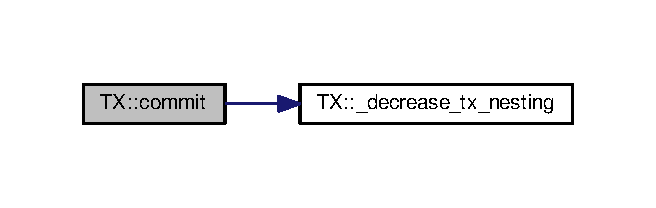
\includegraphics[width=315pt]{class_t_x_a9dde5d356b35e557448e58d260087356_cgraph}
\end{center}
\end{figure}


\index{TX@{TX}!load@{load}}
\index{load@{load}!TX@{TX}}
\paragraph[{\texorpdfstring{load(std\+::shared\+\_\+ptr$<$ O\+S\+T\+M $>$ object)}{load(std::shared_ptr< OSTM > object)}}]{\setlength{\rightskip}{0pt plus 5cm}std\+::shared\+\_\+ptr$<$ {\bf O\+S\+TM} $>$ T\+X\+::load (
\begin{DoxyParamCaption}
\item[{std\+::shared\+\_\+ptr$<$ {\bf O\+S\+TM} $>$}]{object}
\end{DoxyParamCaption}
)}\hypertarget{class_t_x_a1d78262b8831ddd042ed491f2e600e24}{}\label{class_t_x_a1d78262b8831ddd042ed491f2e600e24}


load std\+::shared\+\_\+ptr$<$\+O\+S\+T\+M$>$, returning an std\+::shared\+\_\+ptr$<$\+O\+S\+T\+M$>$ copy of the original pointer, to work with during transaction life time 

Register \hyperlink{class_o_s_t_m}{O\+S\+TM} pointer into S\+TM library


\begin{DoxyParams}{Parameters}
{\em working\+\_\+\+Map\+\_\+collection} & std\+::map, store all the std\+::shared\+\_\+ptr$<$\+O\+S\+T\+M$>$ pointer in the transaction \\
\hline
\end{DoxyParams}


Definition at line \hyperlink{_t_x_8cpp_source_l00155}{155} of file \hyperlink{_t_x_8cpp_source}{T\+X.\+cpp}.


\begin{DoxyCode}
00155                                                        \{
00156 
00157     std::map< int, std::shared\_ptr<OSTM> >::iterator working\_Map\_collection\_Object\_Shared\_Pointer\_Iterator;
00158     \textcolor{comment}{/*}
00159 \textcolor{comment}{     * Check for null pointer !
}
00160 \textcolor{comment}{     * Null pointer can cause segmentation fault!!!
}
00161 \textcolor{comment}{     */}
00162     \textcolor{keywordflow}{if}(\textcolor{keywordtype}{object} == \textcolor{keyword}{nullptr})\{
00163         \textcolor{keywordflow}{throw} std::runtime\_error(std::string(\textcolor{stringliteral}{"[RUNTIME ERROR : NULL POINTER IN LOAD FUNCTION]"}) );
00164     \}
00165 
00166         working\_Map\_collection\_Object\_Shared\_Pointer\_Iterator = working\_Map\_collection.find(object->
      Get\_Unique\_ID());
00167 
00168     \textcolor{keywordflow}{if} (working\_Map\_collection\_Object\_Shared\_Pointer\_Iterator != working\_Map\_collection.end()) \{
00169 
00170         \textcolor{keywordflow}{return} working\_Map\_collection\_Object\_Shared\_Pointer\_Iterator->second->getBaseCopy(
      working\_Map\_collection\_Object\_Shared\_Pointer\_Iterator->second);
00171         
00172     \} \textcolor{keywordflow}{else} \{ \textcolor{keywordflow}{throw} std::runtime\_error(std::string(\textcolor{stringliteral}{"[RUNTIME ERROR : NO OBJECT FOUND LOAD FUNCTION]"}) );\}
00173 \}
\end{DoxyCode}
\index{TX@{TX}!ostm\+\_\+exit@{ostm\+\_\+exit}}
\index{ostm\+\_\+exit@{ostm\+\_\+exit}!TX@{TX}}
\paragraph[{\texorpdfstring{ostm\+\_\+exit()}{ostm_exit()}}]{\setlength{\rightskip}{0pt plus 5cm}void T\+X\+::ostm\+\_\+exit (
\begin{DoxyParamCaption}
{}
\end{DoxyParamCaption}
)}\hypertarget{class_t_x_aa9739c5c2077454c779098db7baefc2b}{}\label{class_t_x_aa9739c5c2077454c779098db7baefc2b}


Delete all map entries associated with the main process. 

ostm\+\_\+exit void, clear all elements from the shared global collections associated with the main process


\begin{DoxyParams}{Parameters}
{\em main\+\_\+\+Process\+\_\+\+Map\+\_\+collection} & std\+::map, store all std\+::shared\+\_\+ptr$<$\+O\+S\+T\+M$>$ from all transaction shared between multiple processes \\
\hline
{\em process\+\_\+map\+\_\+collection} & std\+::map, store all unique id from all transaction within main process DO N\+OT C\+A\+LL T\+H\+IS M\+E\+T\+H\+OD E\+X\+P\+L\+I\+C\+I\+T\+L\+Y!!!!!! W\+I\+LL D\+E\+L\+E\+TE A\+LL P\+R\+O\+C\+E\+SS A\+S\+S\+O\+C\+I\+A\+T\+ED E\+L\+E\+M\+E\+N\+T\+S!!!! \\
\hline
\end{DoxyParams}


Definition at line \hyperlink{_t_x_8cpp_source_l00072}{72} of file \hyperlink{_t_x_8cpp_source}{T\+X.\+cpp}.



Referenced by \hyperlink{_t_m_8cpp_source_l00100}{T\+M\+::\+\_\+\+T\+X\+\_\+\+E\+X\+I\+T()}.


\begin{DoxyCode}
00072                    \{
00073     std::map<int, std::shared\_ptr<OSTM>>::iterator main\_Process\_Map\_collection\_Iterator;
00074      
00075     pid\_t ppid = getppid();
00076     std::map<pid\_t, std::map< int, int >>::iterator process\_map\_collection\_Iterator = 
      TX::process\_map\_collection.find(ppid);
00077     \textcolor{keywordflow}{if} (process\_map\_collection\_Iterator != TX::process\_map\_collection.end()) \{
00078 
00079         \textcolor{keywordflow}{for} (\textcolor{keyword}{auto} current = process\_map\_collection\_Iterator->second.begin(); current != 
      process\_map\_collection\_Iterator->second.end(); ++current) \{
00080             main\_Process\_Map\_collection\_Iterator = TX::main\_Process\_Map\_collection.find(current->first);
00081 
00082             \textcolor{keywordflow}{if} (main\_Process\_Map\_collection\_Iterator != TX::main\_Process\_Map\_collection.end())\{
00083                 \textcolor{comment}{/*}
00084 \textcolor{comment}{                 * Delete element from shared main\_Process\_Map\_collection by object unique key value,
       shared\_ptr will destroy automatically
}
00085 \textcolor{comment}{                 */}
00086                 TX::main\_Process\_Map\_collection.erase(main\_Process\_Map\_collection\_Iterator->first);      
00087             \}
00088         \}
00089         \textcolor{comment}{/*}
00090 \textcolor{comment}{         * Delete from Process\_map\_collection, Main process exits delete association with library
}
00091 \textcolor{comment}{         */}
00092         TX::process\_map\_collection.erase(process\_map\_collection\_Iterator->first);
00093     \}
00094 \}
\end{DoxyCode}


Here is the caller graph for this function\+:\nopagebreak
\begin{figure}[H]
\begin{center}
\leavevmode
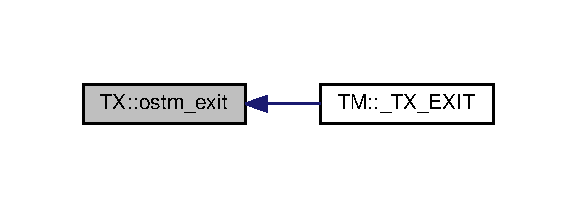
\includegraphics[width=277pt]{class_t_x_aa9739c5c2077454c779098db7baefc2b_icgraph}
\end{center}
\end{figure}


\index{TX@{TX}!store@{store}}
\index{store@{store}!TX@{TX}}
\paragraph[{\texorpdfstring{store(std\+::shared\+\_\+ptr$<$ O\+S\+T\+M $>$ object)}{store(std::shared_ptr< OSTM > object)}}]{\setlength{\rightskip}{0pt plus 5cm}void T\+X\+::store (
\begin{DoxyParamCaption}
\item[{std\+::shared\+\_\+ptr$<$ {\bf O\+S\+TM} $>$}]{object}
\end{DoxyParamCaption}
)}\hypertarget{class_t_x_a7dbcb369aa4a3370b6c6829d278ece5d}{}\label{class_t_x_a7dbcb369aa4a3370b6c6829d278ece5d}


Store transactional changes. 

store void, receive an std\+::shared\+\_\+ptr$<$\+O\+S\+T\+M$>$ object to store the changes within the transaction, depends the user action


\begin{DoxyParams}{Parameters}
{\em working\+\_\+\+Map\+\_\+collection} & std\+::map, store all the std\+::shared\+\_\+ptr$<$\+O\+S\+T\+M$>$ pointer in the transaction \\
\hline
\end{DoxyParams}


Definition at line \hyperlink{_t_x_8cpp_source_l00178}{178} of file \hyperlink{_t_x_8cpp_source}{T\+X.\+cpp}.


\begin{DoxyCode}
00178                                          \{
00179     \textcolor{comment}{/*}
00180 \textcolor{comment}{     * Check for null pointer !
}
00181 \textcolor{comment}{     * Null pointer can cause segmentation fault!!!
}
00182 \textcolor{comment}{     */}
00183     \textcolor{keywordflow}{if}(\textcolor{keywordtype}{object} == \textcolor{keyword}{nullptr})\{
00184         \textcolor{keywordflow}{throw} std::runtime\_error(std::string(\textcolor{stringliteral}{"[RUNTIME ERROR : NULL POINTER IN STORE FUNCTION]"}) );
00185     \}
00186     
00187     std::map< int, std::shared\_ptr<OSTM> >::iterator working\_Map\_collection\_Object\_Shared\_Pointer\_Iterator;
00188 
00189     working\_Map\_collection\_Object\_Shared\_Pointer\_Iterator = working\_Map\_collection.find(object->
      Get\_Unique\_ID());
00190     \textcolor{keywordflow}{if} (working\_Map\_collection\_Object\_Shared\_Pointer\_Iterator != working\_Map\_collection.end()) \{
00191 
00192         working\_Map\_collection\_Object\_Shared\_Pointer\_Iterator->second = object;
00193 
00194     \} \textcolor{keywordflow}{else} \{ std::cout << \textcolor{stringliteral}{"[ERROR STORE]"} << std::endl; \}
00195 \}
\end{DoxyCode}


\subsubsection{Friends And Related Function Documentation}
\index{TX@{TX}!TM@{TM}}
\index{TM@{TM}!TX@{TX}}
\paragraph[{\texorpdfstring{TM}{TM}}]{\setlength{\rightskip}{0pt plus 5cm}friend class {\bf TM}\hspace{0.3cm}{\ttfamily [friend]}}\hypertarget{class_t_x_adf1ccda799ef5c419cb43b8ae55eb45c}{}\label{class_t_x_adf1ccda799ef5c419cb43b8ae55eb45c}
Only \hyperlink{class_t_m}{TM} Transaction Manager can create instance of \hyperlink{class_t_x}{TX} Transaction 

Definition at line \hyperlink{_t_x_8h_source_l00070}{70} of file \hyperlink{_t_x_8h_source}{T\+X.\+h}.



\subsubsection{Member Data Documentation}
\index{TX@{TX}!test\+\_\+counter@{test\+\_\+counter}}
\index{test\+\_\+counter@{test\+\_\+counter}!TX@{TX}}
\paragraph[{\texorpdfstring{test\+\_\+counter}{test_counter}}]{\setlength{\rightskip}{0pt plus 5cm}int T\+X\+::test\+\_\+counter = 0\hspace{0.3cm}{\ttfamily [static]}}\hypertarget{class_t_x_a25838234aab99ae891a90eb8623a8b3c}{}\label{class_t_x_a25838234aab99ae891a90eb8623a8b3c}

\begin{DoxyParams}{Parameters}
{\em test\+\_\+counter} & int O\+N\+LY F\+OR T\+E\+S\+T\+I\+N\+G!!!\\
\hline
{\em static} & Global counter for rollback \\
\hline
\end{DoxyParams}


Definition at line \hyperlink{_t_x_8h_source_l00078}{78} of file \hyperlink{_t_x_8h_source}{T\+X.\+h}.



Referenced by \hyperlink{_t_x_8cpp_source_l00202}{commit()}, and \hyperlink{_t_x_8cpp_source_l00324}{get\+Test\+\_\+counter()}.



The documentation for this class was generated from the following files\+:\begin{DoxyCompactItemize}
\item 
T\+X.\+h\item 
T\+X.\+cpp\end{DoxyCompactItemize}

%--- End generated contents ---

% Index
\newpage
\phantomsection
\clearemptydoublepage
\addcontentsline{toc}{section}{Index}
\printindex

\end{document}
